\section{Προδιαγραφή μεθόδου υλοποίησης και χρονοπρογραμματισμός} \label{section:3-8-implementation-methodology-specification}

Κατά τον χρονοπρογραμματισμό ακολουθήθηκαν οι τακτικές που ορίζει το Scrum. Το συνολικό προγραμματιστικό έργο χωρίστηκε σε επιμέρους, διακριτούς στόχους και κάθε στόχος αντιστοιχήθηκε σε ένα Sprint. Τα Sprints αποτελούνται από επιμέρους διαχωρισμό της εργασίας σε epic tasks. Σε αυτό το στάδιο χρονοπρογραμματισμού δεν έγινε αναλυτικότερη περιγραφή των επιμέρους tasks, κάθε epic χωρίστηκε σε tasks κατά το αρχικό στάδιο της υλοποίησης του.

Ως σημαντικότερος στόχος της ανάπτυξης ορίζεται η δημιουργία ενός ελάχιστου βιώσιμου προϊόντος (Minumum Viable Product - MVP). Σε αυτό τον στόχο περιλαμβάνονται πιο στοιχειώδεις λειτουργίες μίας πλατφόρμας επικοινωνίας οι οποίες την κάνουν χρήσιμη, η δυνατότητα εγγραφής, δημιουργίας θεμάτων και μηνυμάτων και ανάγνωσης του υπάρχοντος περιεχομένου. Επειδή ο στόχος αυτός περιέχει από μόνος του σημαντική περιπλοκότητα και δυσκολία κρίθηκε αναγκαίος ο περαιτέρω διαχωρισμός του σε τρία Sprints.

Στο πρώτο Sprint ορίστηκε ο στόχος της δημιουργίας μίας βάσης κώδικα (codebase), της εξοικείωσης με τα προγραμματιστικά εργαλεία του οικοσυστήματος των DApps και της επιτυχής δημιουργίας του πρώτου contract. Στο δεύτερο Sprint ο στόχος ορίστηκε ως η δημιουργία των τεχνικών χαρακτηριστικών που αφορούν τους χρήστες της πλατφόρμας και που οι ίδιοι (οι χρήστες) έχουν συνηθίσει να περιμένουν από μία τέτοια πλατφόρμα. Στο τρίτο Sprint συμπεριλήφθηκαν τα τεχνικά χαρακτηριστικά που απομένουν ώστε να δημιουργηθεί το MVP.

Τα επόμενα τρία Sprints χτίζουν διαδοχικά πάνω στην υπάρχουσα δουλειά και υποδομή. Στο τέταρτο μέρος εργασίας ως στόχος ορίστηκε η προσθήκη των χαρακτηριστικών ψηφοφορίας πάνω στα μηνύματα και δημιουργίας ψηφοφοριών θεμάτων (polls). Το επόμενο Sprint περιλαμβάνει εργασίες δημιουργίας υποδομής και την πρώτη ημι-δημόσια εγκατάσταση της εφαρμογής σε περιβάλλον δοκιμής. Το τελευταίο Sprint αποτελεί το τελικό προϊόν και περιέχει tasks σχετικά με την δημιουργία κοινοτήτων και την beta εγκατάσταση της εφαρμογής.

Εποπτικά, η διαδικασία της υλοποίησης περιγράφεται στο παρακάτω σχήμα (σχήμα \ref{figure:3.8.implementation-methodology-specification-sprints}).

\begin{figure}[H]
    \centering
    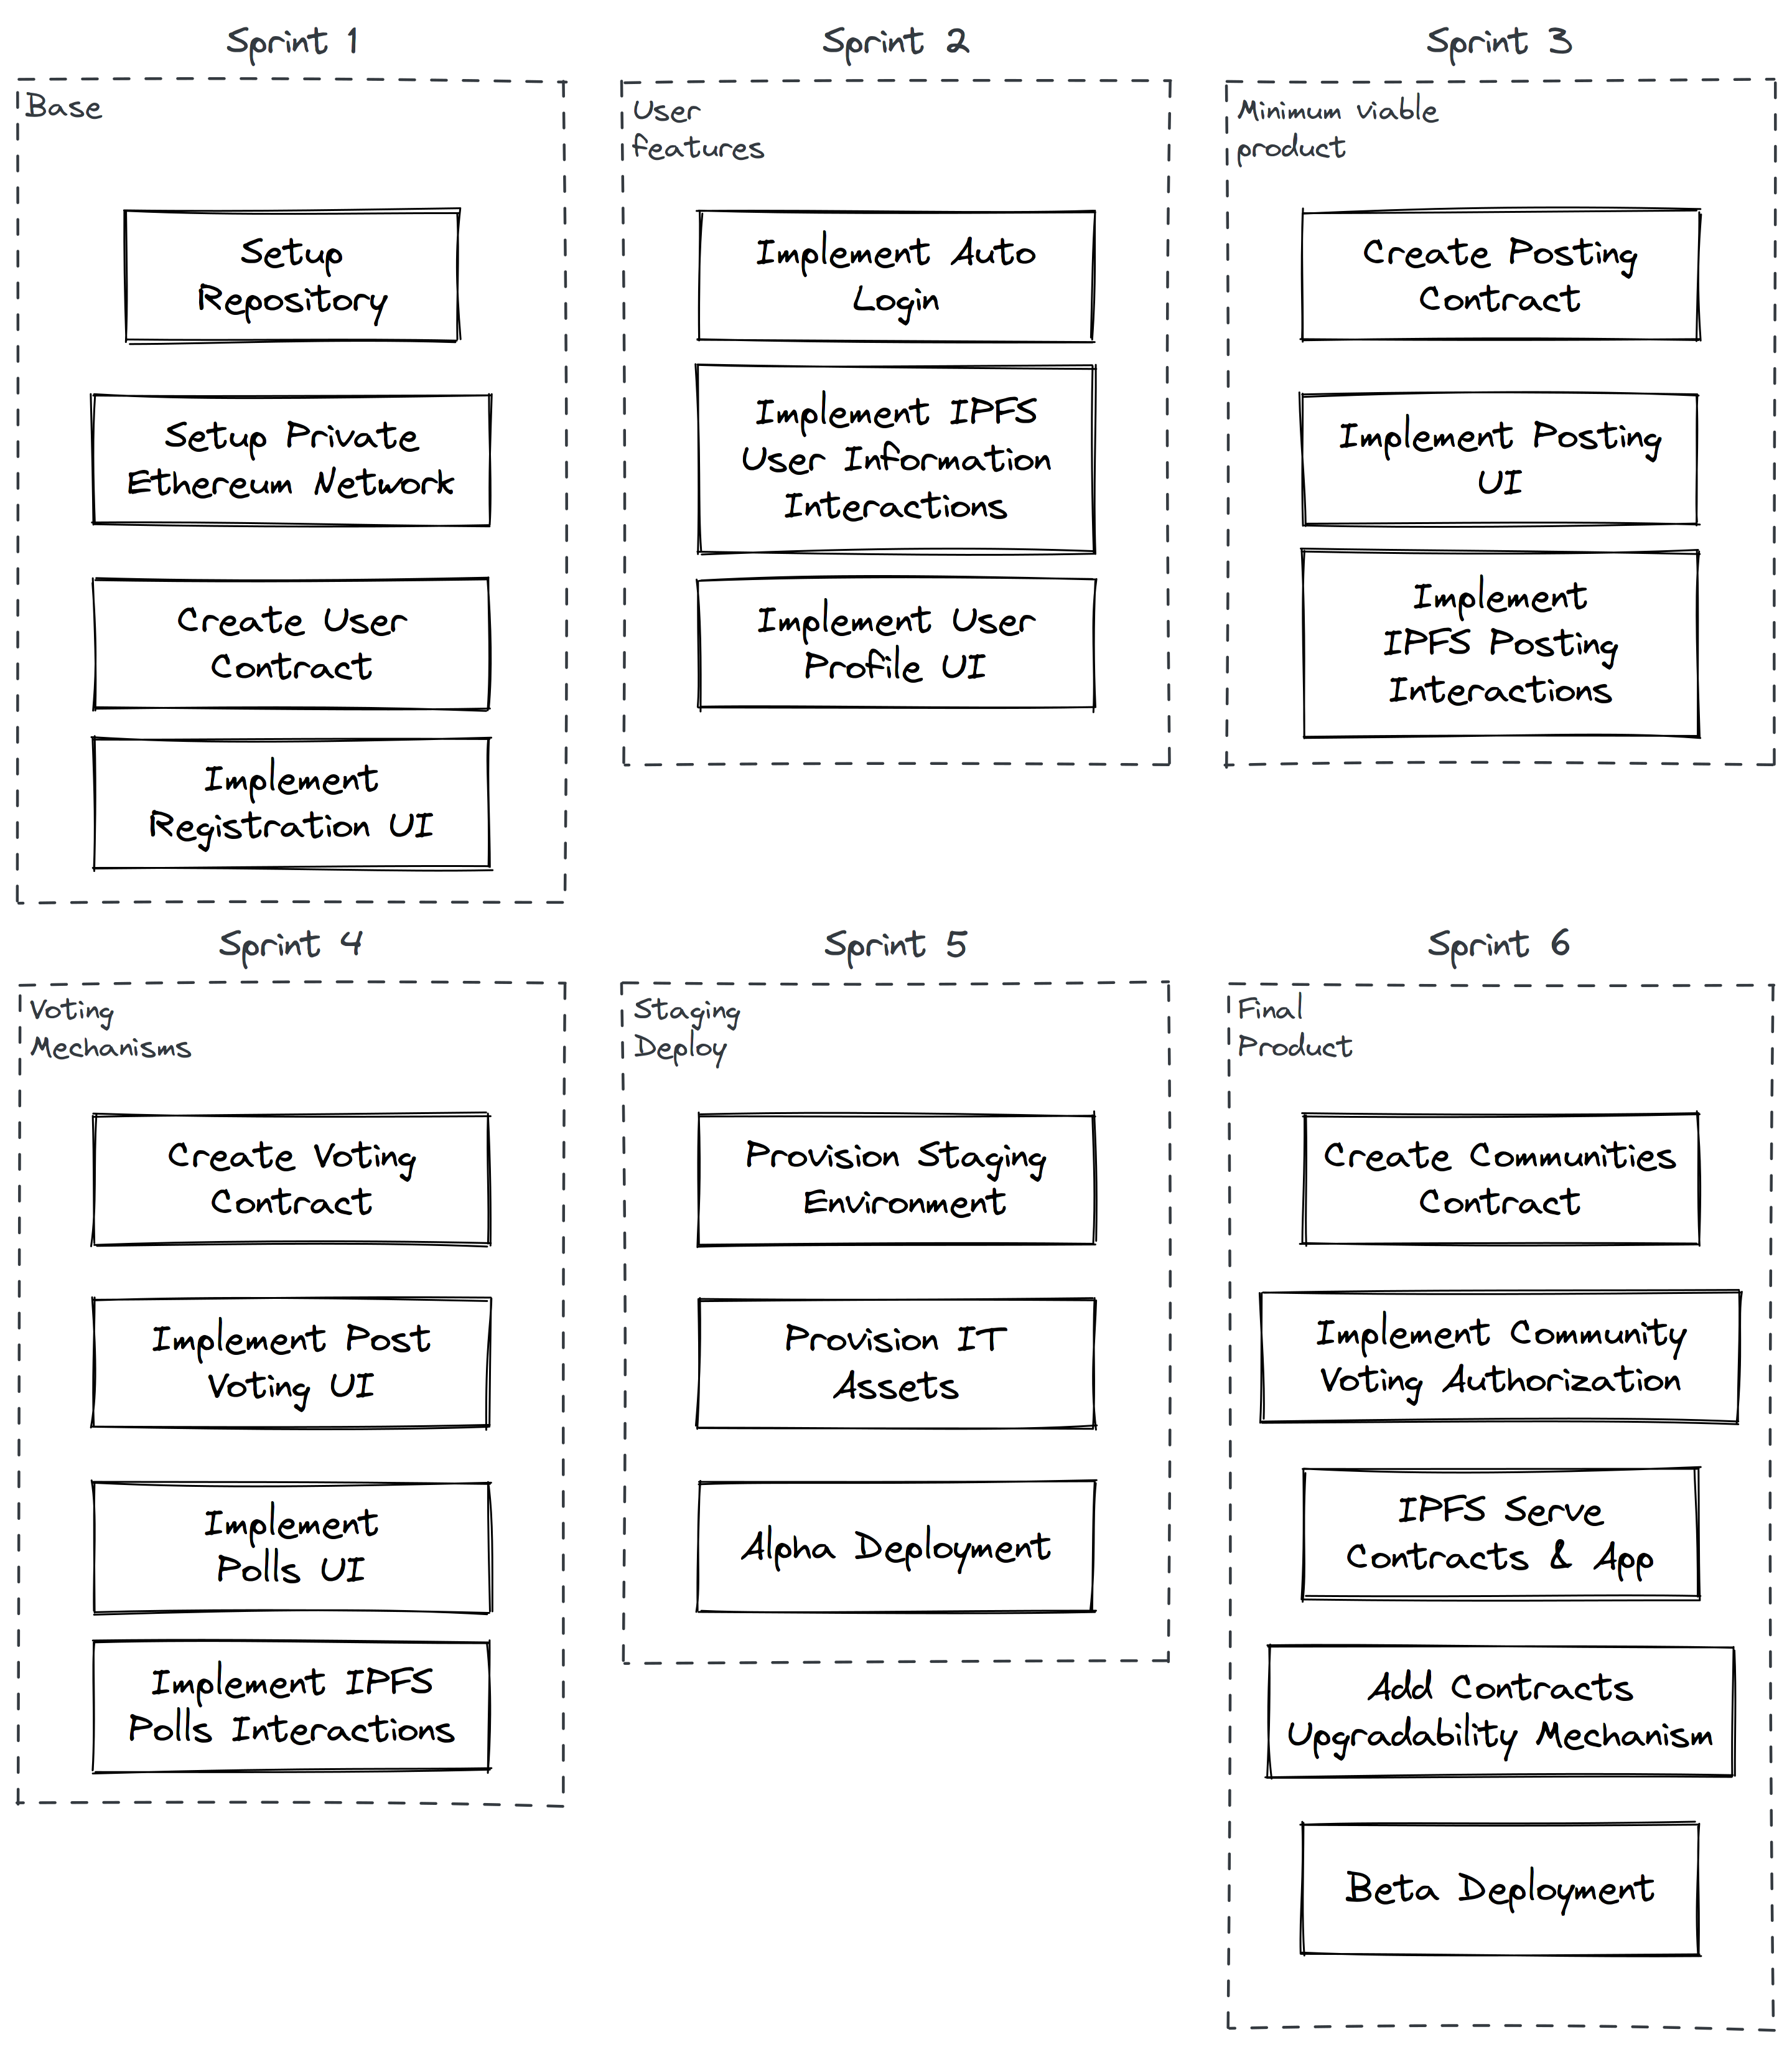
\includegraphics[width=.8\textwidth]{assets/figures/chapter-3/3.8.implementation-methodology-specification-sprints.png}
    \caption{Διαχωρισμός σε sprints}
    \label{figure:3.8.implementation-methodology-specification-sprints}
\end{figure}
